\documentclass[12pt,t]{beamer}
% \documentclass[t]{beamer}
\usepackage[utf8]{inputenc}
\usepackage[spanish]{babel}
\usepackage{verbatim}
\usepackage{hyperref}
\hypersetup{colorlinks=true}
\usepackage{amsfonts,amssymb,amsmath,amsthm,wasysym}
\usepackage{listings}
\usepackage[T1]{fontenc}        
\usepackage{accents}

%
\usetheme[hideothersubsections,left]{Marburg}
\usecolortheme{sidebartab}
\useinnertheme[shadow]{rounded}
\setbeamertemplate{navigation symbols}{}
% \useoutertheme[footline=empty,subsection=true,compress]{infolines}
% \useoutertheme[footline=empty,subsection=true,compress]{miniframes}
%\usefonttheme{serif}

\setbeamertemplate{caption}[numbered]

\newcommand{\red}[1]{\textcolor{red}{#1}}
\newcommand{\green}[1]{\textcolor{green}{#1}}
\newcommand{\blue}[1]{\textcolor{blue}{#1}}
\newcommand{\gray}[1]{\textcolor{gray}{#1}}
\renewcommand{\emph}[1]{{\color{red}#1}}

\setbeamertemplate{frametitle}
{\begin{centering}
\medskip
\color{blue}
\textbf{\insertframetitle}
\medskip
\end{centering}
}
\usecolortheme{rose}
\usecolortheme{dolphin}
\mode<presentation>

\newcommand{\CC}{\mathbb{C}}
\newcommand{\RR}{\mathbb{R}}
\newcommand{\ZZ}{\mathbb{Z}}
\newcommand{\NN}{\mathbb{N}}
\newcommand{\QQ}{\mathbb{Q}}
\renewcommand{\leq}{\leqslant}
\renewcommand{\geq}{\geqslant}

\theoremstyle{plain}
\newtheorem{teorema}{Teorema}
\newtheorem{formula}[theorem]{Fórmula}
\theoremstyle{definition}
\newtheorem{pregunta}{Pregunta}
\newtheorem{definicio}{Definició}

\title[\red{Matemáticas III GINF}]{}

\author[]{Ricardo Alberich}


\date{}


\begin{document}
\beamertemplatedotitem


\lstset{backgroundcolor=\color{green!50}}
\lstset{breaklines=true}
\lstset{basicstyle=\ttfamily}


\begin{frame}
\vfill
\begin{center}
\gray{\Huge Matemáticas III GINF}\\[3ex]
\Large Curso 2018-19\\[3ex]
%\blue{(Ostres, un déjà vu!)}
\end{center}
\vfill
\end{frame}


\section{Presentación}

\subsection{Dónde estamos}
\begin{frame}
\frametitle{¿Quiénes somos?}
\vspace*{-0.2cm}

%\begin{minipage}[c]{0.45\linewidth}

%\begin{center}
\red{GRUPO 1 GG y Medianos 1 y 2:}\\ \href{https://www.uib.es/es/personal/ABDI0ODk/}{R. Alberich} y \href{https://www.uib.es/es/personal/ABjI5MTE5Mw/}{Eloy Sousa} (profesor asociado)\medskip

% 
% 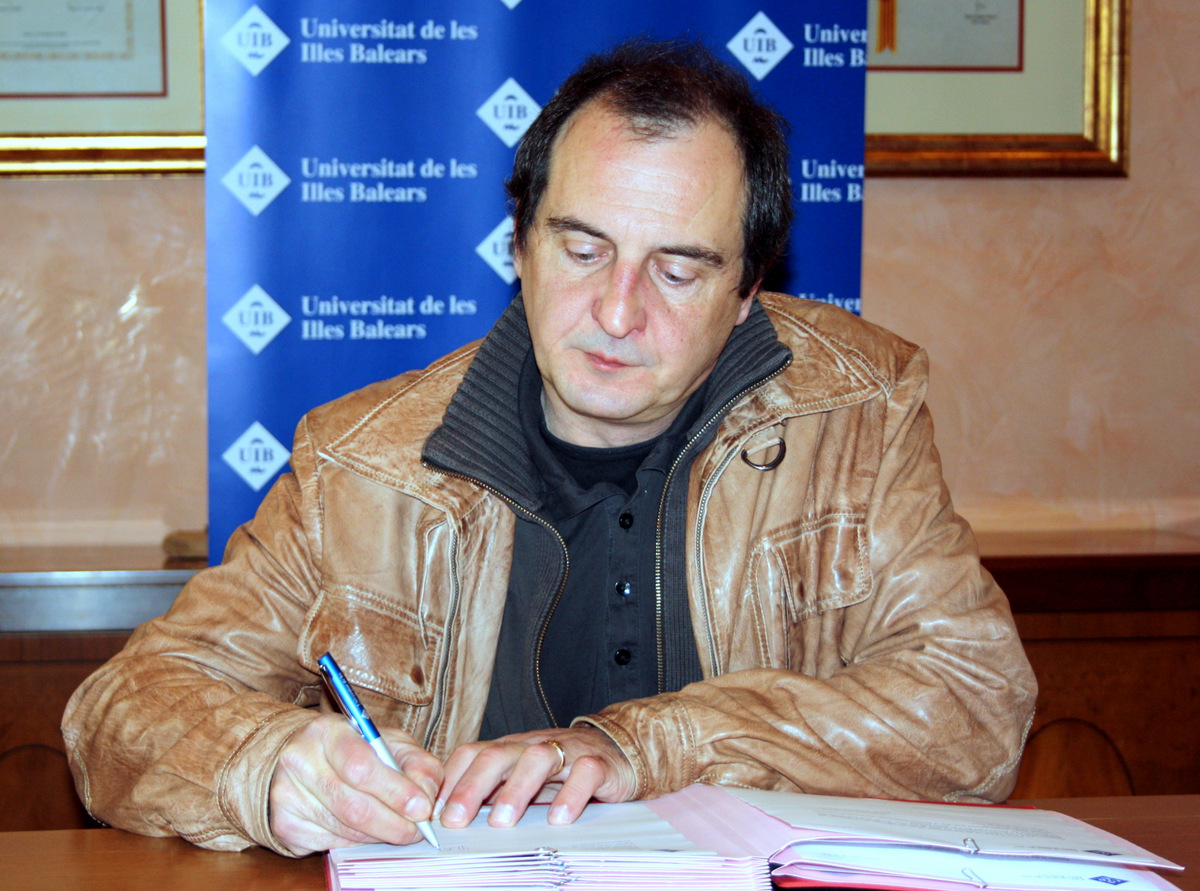
\includegraphics[width=0.7\linewidth]{196022_img_009_ricardo_alberich_marti.jpg}\\
% 
\includegraphics[height=3cm]{image.jpg}\\
% \medskip

\red{Despacho} 256,\\
 Ed. Anselm Turmeda, orimer piso al lado de secretaría.
\medskip

\red{Tel.} (971 25) 3203
\medskip

\red{Tutorías:} Viernes, de 12 a 13 (o con cita previa a convenir)
%\end{center}
\vspace*{\fill}

\
%\end{minipage}\quad




\end{frame}
%\end{document}

\subsection{Objetivos}
\begin{frame}
\frametitle{Objetivos}
\medskip

Introducción a la probabilidad, estadística inferencial, el análisis de datos y si se puede a la ciencia de datos.
\medskip

\begin{itemize}
\item Probabilidad
\item Estimación de parámetros
\item Intervalos de confianza
\item Contrastes de hipótesis
\item Análisis de la varianza
\item Regresión lineal simple y múltiple
\item Otras metodología del aprendizaje estadístico  y del análisis de datos
\item \ldots\pause
\item Lo haremos con R y sus amigos
\item Aprenderemos a a escribir informes técnicos con datos y gráficos.

\end{itemize}


\end{frame}

\subsection{Actividades}
\begin{frame}
\frametitle{Actividades}

\red{Clases en grupo grande:}
\smallskip

Pues... el profesor hablará y vosotros haréis las actividades  que se os propongan.\bigskip

\red{Clases en grupo mediano:} Se alternaran,
\smallskip

\begin{itemize}
\item Talleres de resolución ejercicios/problemas

\item Talleres de prácticas de análisis de datos con R
\end{itemize}
\bigskip
\pause

\red{Trabajo en casa} ($\sim$ 4 horas semanales):
\smallskip

Estudiar, resolver problemas, estudiar los temas de R..... contestar cuestionarios, \ldots
\smallskip

\end{frame}


\subsection{Evaluación}

\begin{frame}
\frametitle{Evaluación}
\medskip

\href{https://estudis.uib.cat/guia_docent/2018-19/20305/1/es/guia_docent.pdf}{\blue{Ver y leer (obligatorio) la guía docente de la asignatura.}}
\end{frame}

%\end{document}

\subsection{Bibliografía}

\begin{frame}
\frametitle{Bibliografía}
\begin{itemize} 

\item Presentaciones y apuntes complementarios, en Aula Digital o en el github de los profesores.
\medskip

\item \href{https://www.uib.es/es/personal/ABDI0ODk/}{R. Alberich}, \href{https://www.uib.es/es/personal/ABDMyNjc/}{A. Mir}, \href{https://www.uib.es/es/personal/ABDUyODM/}{F. Rosselló} Más lecciones de R y el MOOC (enlaces en Aula Digital).
\medskip

\item Más bibliografía en Aula Digital.
%\item  J. S. Milton. \textsl{Estadística para Biología y Ciencias de la Salud}, $3^{\mathrm{a}}$ edición
%ampliada. McGraw Hill Interamericana (2007). 
\medskip

%\item D. Peña. \textsl{Análisis Multivariante de Datos}. McGraw Hill Interamericana (2002)
\end{itemize}

\end{frame}


\subsection{Consejos finales}

\begin{frame}
\frametitle{Consejos finales}

\begin{itemize}
\item Acceder a  Aula Digital  cuanto antes, esta semana ya haremos actividades y foros.

\item Llevar calculadora científica, ordenador o móvil.

\item Venid a clase de teoría con las presentaciones impresas o un medio digital para leerlas.

\item Consultad el \emph{Calendario de la asignatura en Aula Digital}, es lo  que nos servirá de cronograma detallado.

\item Consultad el \emph{Tablón de Anuncios de Aula Digital}, es la manera básica de comunicarnos con nosotros para problemas de logística.

\item Procurar  hacer todas las tareas que os mandemos, y cuanto antes mejor.

\end{itemize}

\end{frame}


\begin{frame}
\frametitle{Consejos finales}

No dediquéis  más tiempo del necesario a la asignatura
\medskip

\begin{itemize}
% \item No repetiu tests innecessàriament
% \medskip
\item En esta asignatura hay que estudiar bastante.
\medskip
%\item El exercicis per fer a casa estan pensats per 1 hora de feina quinzenal si se sap la matèria (i R)\medskip
\item Emplead los recursos de Aula Digital.
\item Consultad cualquier duda.
\item Preguntad en los foros de Aula Digital
\item Pedid tutorías.
\item Contestar dudas de compañeros en los foros de Aula Digital.
\end{itemize}
\vspace*{1cm}
\pause

\red{Venga pues, haced los primeros problemas de conteo y de probabilidad}.

\end{frame}





\end{document}



